\section{Koncept} \label{Endelig koncept}
Illustration af det endelige konceptforslag ses i figur \ref{fig: endelig koncept}. Konceptet er konceptforlag 10 ($\protect\mathcolor{BrickRed}{\clubsuit}$) fra afsnit \ref{Mekanisk system - vurdering} med et kamera til kalibrering af emne placering og en touchskærm som brugerflade. Kameraet og touchskærmen er valgt i bilag \ref{Bilag - morf til kontrolsystem}, og tages højde for i den videre udvikling af de mekaniske dele. 

\begin{figure}[H]
    \centering
    \includegraphics[width=0.7\linewidth]{Sections/5 Konceptgenerering/Media/Endelige løsning.png}
    \caption{Koncept 10 $\protect\mathcolor{BrickRed}{\clubsuit}$. }
    \label{fig: endelig koncept}
\end{figure} \plainbreak{-0.5}

Konceptet videreudvikles i følgende del, hvor mekanismen der skal sætte dråber undersøges yderligere og der foretages valg af bevægelsesmekanisme til den lineære bevægelse. Dette sker med udgangspunkt i designspecifikationer og ufravigelige krav fra afsnit \ref{Endelige kravspecifikationer}.


%Det endelige koncept rejser en række tekniske problemstillinger, der kræver nærmere undersøgelse, herunder mekanismen, som er ansvarlig for at afsætte dråber, hvordan denne mekanisme fungerer, og hvordan den skal fungere i forhold til konceptet. Derefter, hvordan man opnår den højeste præcision ved lineær bevægelse, og forskellige måder at presse på emnet er også blandt disse spørgsmål.


%Hvordan specifikt "åbne/lukke" mekanisme skal fungere er nok det største nye spørgsmål. Derefter, hvordan man opnår den højeste præcision ved lineær bevægelse og forskellige måder at presse på emnet.

\begin{comment}
\begin{figure}[H]
    \caption{Billede af det endelige koncept samt tabel over de delfunktioner den består af.}
    \label{fig:Endelige konceptdesign}
    \small
    \begin{tabularx}{\textwidth}{|Y|Y|Y|Y|p{1pt}|Y|Y|} 
        \hline
        \rowcolor{aaublue}\multicolumn{4}{|c}{\textcolor{white}{\textbf{Mekanisksystem}}} & & \multicolumn{2}{c|}{\textcolor{white}{\textbf{Kontrolsystem }}} \\ \hline
        \rowcolor{lightgray!30} Bevægelse & Sætte prikker & Indspænding & Understøttelse & & Brugerflade & Formanalyse \\ \hline
        \includegraphics[width=0.80\linewidth]{Sections/5 Konceptgenerering/Media/lineær.png} & 
        \includegraphics[width=0.80\linewidth]{Sections/5 Konceptgenerering/Media/åbnelukke.png} &
        \includegraphics[width=0.80\linewidth]{Sections/5 Konceptgenerering/Media/Press på emnet.png} &
        \includegraphics[width=0.80\linewidth]{Sections/5 Konceptgenerering/Media/Understøttelse plade.png} & &
        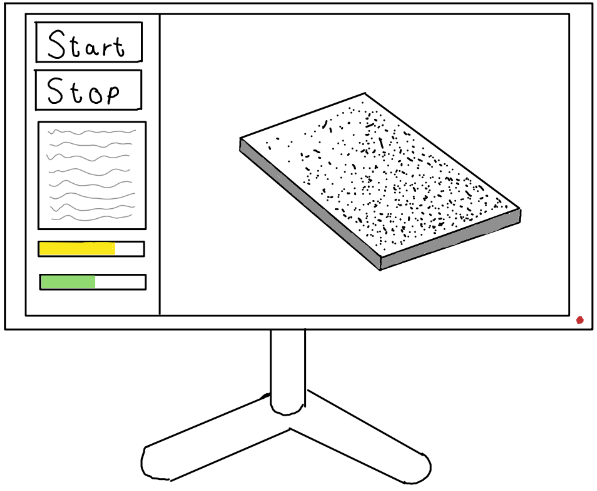
\includegraphics[width=0.80\linewidth]{Sections/5 Konceptgenerering/Media/Computer.png} & 
        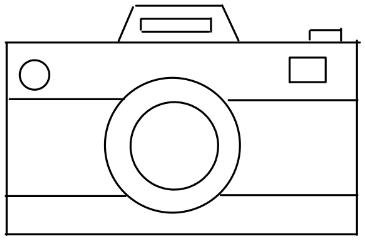
\includegraphics[width=0.80\linewidth]{Sections/5 Konceptgenerering/Media/Kamera.png} \\ \hline
        
        \rowcolor{aaublue}\multicolumn{7}{|c|}{\textcolor{white}{\textbf{Endelig koncept}}} \\ \hline
        \multicolumn{7}{|c|}{\includegraphics[width=0.80\linewidth]{Sections/5 Konceptgenerering/Media/Endelige løsning.png}} \\ \hline
    \end{tabularx}
\end{figure}
  
\end{comment}
